\documentclass[aspectratio=169]{beamer}

% Use the Conesa Group theme
\usetheme{ConesaGroup}

% Package for better font rendering
\usepackage{lmodern}
\usepackage{microtype}

% Package for graphics
\usepackage{graphicx}
\graphicspath{{assets/}{src/assets/}}

% Package for tables with colors
\usepackage{colortbl}

% Package for mathematics
\usepackage{amsmath}
\usepackage{amssymb}

% Package for bibliography and citations
\usepackage[natbib=true,backend=biber,style=numeric,sorting=none,autocite=superscript]{biblatex}
\addbibresource{ai_workshop_references.bib}

% Package for code listings
\usepackage{listings}
\lstset{
  basicstyle=\ttfamily\small,
  keywordstyle=\color{conesaTeal}\bfseries,
  commentstyle=\color{conesaGray},
  stringstyle=\color{conesaOrange},
  numbers=left,
  numberstyle=\tiny\color{conesaGray},
  numbersep=5pt,
  frame=single,
  breaklines=true,
  breakatwhitespace=true,
}

% Package for TikZ diagrams
\usepackage{tikz}
\usetikzlibrary{shapes,arrows,arrows.meta,positioning,shadows,calc,decorations.markings}

% Custom colors for agent diagrams
\definecolor{reasonPrimary}{HTML}{006D77}
\definecolor{reasonFill}{HTML}{E0F2F1}
\definecolor{actPrimary}{HTML}{1D4ED8}
\definecolor{actLMFill}{HTML}{DBEAFE}
\definecolor{actEnvFill}{HTML}{E0E7FF}
\definecolor{reactPrimary}{HTML}{B45309}
\definecolor{reactLMFill}{HTML}{FEF3C7}
\definecolor{reactEnvFill}{HTML}{DCFCE7}

% Title information
\title{How to Make Your Science Easier with AI Support}
\subtitle{}
\author[T. Liu]{Tianyuan Liu}
\date{October 3rd, 2025}

% Institute
\institute[University]{%
  \begin{flushleft}
    \textbf{Date:} October 3rd, 2025\\
    \textbf{Time:} 10:00--12:00\\
    \textbf{Location:} I2SysBio Seminar Room\\[1ex]
    \small by our PhD student: \textbf{Tianyuan Liu}
  \end{flushleft}%
}

\begin{document}

% Title page
\begin{frame}[plain]
  \titlepage
\end{frame}

% Table of contents
\begin{frame}{Outline}
  \tableofcontents[hideallsubsections]
\end{frame}

% Workshop Structure Overview
\begin{frame}{Workshop Structure}
  \begin{columns}[T]
    \begin{column}{0.48\textwidth}
      \centering
      \large\bfseries
      \textcolor{conesaTeal}{What We'll Cover}

      \vspace{0.5cm}
      \normalsize

      \begin{enumerate}
        \item \textbf{AI Agents Fundamentals}\\
        \small ReAct, MCP, Tools
        
        \vspace{0.3cm}
        
        \item \textbf{Context Engineering}\\
        \small Guiding AI effectively
        
        \vspace{0.3cm}
        
        \item \textbf{Responsible AI}\\
        \small Best practices \& quality
        
        \vspace{0.3cm}
        
        \item \textbf{Future Directions}\\
        \small What's next
      \end{enumerate}
    \end{column}
    \begin{column}{0.48\textwidth}
      \centering
      \large\bfseries
      \textcolor{conesaOrange}{Live Demos}

      \vspace{0.5cm}
      \normalsize

      \begin{itemize}
        \item \textbf{Demo 1}: Research slides\\
        \small LaTeX generation from papers
        
        \vspace{0.3cm}
        
        \item \textbf{Demo 2}: CV generation\\
        \small Context engineering in action
        
        \vspace{0.3cm}
        
        \item \textbf{Demo 3}: React website\\
        \small Unit testing \& CI/CD
      \end{itemize}
    \end{column}
  \end{columns}

  \vspace{0.5cm}
  \centering
  \normalsize
  \textbf{Hands-on + Theory} for practical AI-assisted research
\end{frame}

% Section: Introduction to AI-Assisted Development
\section{Introduction to AI-Assisted Development}

\begin{frame}{LLM vs. AI Agent}
  \begin{columns}[T]
    \begin{column}{0.48\textwidth}
      \centering
      \large\bfseries
      \textcolor{conesaOrange}{Large Language Model}

      \vspace{0.5cm}
      \normalsize

      \begin{itemize}
        \item Cannot use tools
      \end{itemize}

      \vspace{0.3cm}
      \textbf{Example:} ChatGPT (basic mode)
    \end{column}
    \begin{column}{0.48\textwidth}
      \centering
      \large\bfseries
      \textcolor{conesaTeal}{AI Agent}

      \vspace{0.5cm}
      \normalsize

      \begin{itemize}
        \item \textbf{Tools}: Execute actions
        \item \textbf{Memory}: Context retention
        \item \textbf{Planning}: Multi-step tasks
      \end{itemize}

      \vspace{0.3cm}
      \textbf{Example:} Cursor, Gemini CLI
    \end{column}
  \end{columns}

  \vspace{0.5cm}
  \centering
  \normalsize
  \textbf{Agent = LLM + Tools + Memory + Planning}
\end{frame}

\begin{frame}{Reason Only and Act Only}
  \begin{columns}[T]
    \begin{column}{0.48\textwidth}
      \centering
      \begin{minipage}[t][4.8cm][c]{\linewidth}
        \centering
        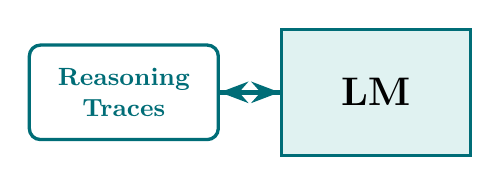
\begin{tikzpicture}[
          box/.style={rectangle, draw=reasonPrimary, fill=reasonFill, minimum width=2.4cm, minimum height=1.6cm, very thick},
          note/.style={rounded corners, draw=reasonPrimary, fill=white, minimum width=2.4cm, minimum height=1.2cm, very thick, text=reasonPrimary, font=\small\bfseries, align=center},
          flow/.style={->, >=Stealth, ultra thick, draw=reasonPrimary}
        ]
          \node[box] (lm1) {\Large\textbf{LM}};
          \node[note] (trace) at (-3.2,0) {Reasoning\\Traces};
          \draw[flow] (trace.east) -- (lm1.west);
          \draw[flow] (lm1.west) -- (trace.east);
        \end{tikzpicture}
      \end{minipage}
      \vspace{0.3cm}
      {\color{reasonPrimary}\textbf{Reason Only}}
    \end{column}
    \begin{column}{0.48\textwidth}
      \centering
      \begin{minipage}[t][4.8cm][c]{\linewidth}
        \centering
        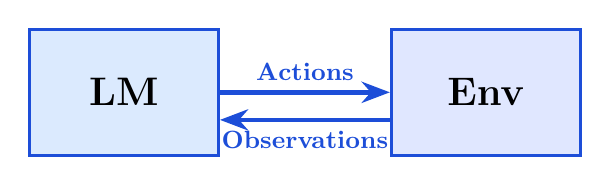
\begin{tikzpicture}[
          boxLM/.style={rectangle, draw=actPrimary, fill=actLMFill, minimum width=2.4cm, minimum height=1.6cm, very thick},
          boxEnv/.style={rectangle, draw=actPrimary, fill=actEnvFill, minimum width=2.4cm, minimum height=1.6cm, very thick},
          flow/.style={->, >=Stealth, ultra thick, draw=actPrimary},
          label/.style={font=\small\bfseries, text=actPrimary}
        ]
          \node[boxLM] (lm2) at (0,0) {\Large\textbf{LM}};
          \node[boxEnv] (env2) at (4.6,0) {\Large\textbf{Env}};
          \draw[flow] (lm2.east) -- node[label, pos=0.5, above] {Actions} (env2.west);
          \draw[flow, transform canvas={yshift=-0.35cm}] (env2.west) -- node[label, pos=0.5, below] {Observations} (lm2.east);
        \end{tikzpicture}
      \end{minipage}
      \vspace{0.3cm}
      {\color{actPrimary}\textbf{Act Only}}
    \end{column}
  \end{columns}
\end{frame}

\begin{frame}{ReAct (Reason + Act)}
  \centering
  \begin{minipage}[t][4.8cm][c]{0.9\textwidth}
    \centering
    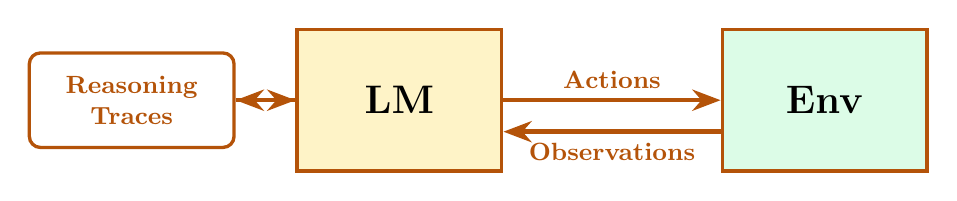
\begin{tikzpicture}[
      boxLM/.style={rectangle, draw=reactPrimary, fill=reactLMFill, minimum width=2.6cm, minimum height=1.8cm, very thick},
      boxEnv/.style={rectangle, draw=reactPrimary, fill=reactEnvFill, minimum width=2.6cm, minimum height=1.8cm, very thick},
      note/.style={rounded corners, draw=reactPrimary, fill=white, minimum width=2.6cm, minimum height=1.2cm, very thick, text=reactPrimary, font=\small\bfseries, align=center},
      flow/.style={->, >=Stealth, ultra thick, draw=reactPrimary},
      label/.style={font=\small\bfseries, text=reactPrimary}
    ]
      \node[boxLM] (lm) at (0,0) {\Large\textbf{LM}};
      \node[note] (trace) at (-3.4,0) {Reasoning\\Traces};
      \node[boxEnv] (env) at (5.4,0) {\Large\textbf{Env}};
      \draw[flow] (trace.east) -- (lm.west);
      \draw[flow] (lm.west) -- (trace.east);
      \draw[flow] (lm.east) -- node[label, pos=0.5, above] {Actions} (env.west);
      \draw[flow, transform canvas={yshift=-0.4cm}] (env.west) -- node[label, pos=0.5, below] {Observations} (lm.east);
    \end{tikzpicture}
  \end{minipage}
  \vspace{0.3cm}
  {\color{reactPrimary}\textbf{ReAct (Reason + Act)}}
\end{frame}

\begin{frame}{Why Do We Need MCP?}
  \begin{block}{The Missing Link}
    ReAct requires \textbf{tools} to interact with the environment --- but how does the LM find and use them?
  \end{block}

  \vspace{0.5cm}

  \begin{columns}[T]
    \begin{column}{0.48\textwidth}
      \centering
      \large\bfseries
      \textcolor{conesaOrange}{The Challenge}

      \vspace{0.3cm}
      \normalsize

      \begin{itemize}
        \item Each tool has unique API
        \item Manual integration required
        \item LM can't discover tools
      \end{itemize}
    \end{column}
    \begin{column}{0.48\textwidth}
      \centering
      \large\bfseries
      \textcolor{conesaTeal}{The Solution: MCP}

      \vspace{0.3cm}
      \normalsize

      \begin{itemize}
        \item Standardized protocol
        \item Auto tool discovery
        \item LM acts with environment
      \end{itemize}
    \end{column}
  \end{columns}

  \vspace{0.5cm}
  \centering
  \normalsize
  \textbf{MCP} = The bridge enabling ReAct to work in practice
\end{frame}

\begin{frame}{API vs MCP: Before and After}
  \begin{columns}[T]
    \begin{column}{0.48\textwidth}
      \centering
      {\large\bfseries\textcolor{conesaOrange}{Before MCP}}

      \vspace{0.3cm}
      \begin{tikzpicture}[scale=0.65, transform shape, node distance=1.0cm and 1.3cm, every node/.style={font=\small}]
        \node[draw, fill=conesaLightGray!60, rounded corners, minimum width=1.8cm, minimum height=0.9cm, thick] (llmA) {LLM};
        \node[draw, fill=white, rounded corners, minimum width=1.8cm, minimum height=0.8cm, below left=of llmA] (apiA) {API 1};
        \node[draw, fill=white, rounded corners, minimum width=1.8cm, minimum height=0.8cm, below=of llmA] (apiB) {API 2};
        \node[draw, fill=white, rounded corners, minimum width=1.8cm, minimum height=0.8cm, below right=of llmA] (apiC) {API 3};
        \draw[->, thick] (llmA) -- node[midway, sloped, above, font=\scriptsize] {Unique API} (apiA);
        \draw[->, thick] (llmA) -- node[midway, right, font=\scriptsize] {Unique API} (apiB);
        \draw[->, thick] (llmA) -- node[midway, sloped, above, font=\scriptsize] {Unique API} (apiC);
      \end{tikzpicture}

      \vspace{0.5cm}
      \textbf{Traditional API}

      \small
      \textit{You write code}
    \end{column}
    \begin{column}{0.48\textwidth}
      \centering
      {\large\bfseries\textcolor{conesaTeal}{After MCP}}

      \vspace{0.3cm}
      \begin{tikzpicture}[scale=0.65, transform shape, node distance=1.0cm and 1.3cm, every node/.style={font=\small}]
        \node[draw, fill=conesaLightGray!60, rounded corners, minimum width=1.8cm, minimum height=0.9cm, thick] (llmB) {LLM};
        \node[draw, fill=conesaTeal!20, rounded corners, minimum width=2.2cm, minimum height=0.9cm, thick, below=of llmB] (mcp) {Model Context Protocol};
        \node[draw, fill=white, rounded corners, minimum width=1.8cm, minimum height=0.8cm, below left=of mcp] (toolA) {API 1};
        \node[draw, fill=white, rounded corners, minimum width=1.8cm, minimum height=0.8cm, below=of mcp] (toolB) {API 2};
        \node[draw, fill=white, rounded corners, minimum width=1.8cm, minimum height=0.8cm, below right=of mcp] (toolC) {API 3};
        \draw[->, thick] (llmB) -- node[midway, right, font=\scriptsize] {Unified API} (mcp);
        \draw[->, thick] (mcp) -- node[midway, sloped, above, font=\scriptsize] {Auto wiring} (toolA);
        \draw[->, thick] (mcp) -- node[midway, right, font=\scriptsize] {Auto wiring} (toolB);
        \draw[->, thick] (mcp) -- node[midway, sloped, above, font=\scriptsize] {Auto wiring} (toolC);
      \end{tikzpicture}

      \vspace{0.5cm}
      \textbf{MCP}

      \small
      \textit{AI uses tools}
    \end{column}
  \end{columns}

  \vspace{0.4cm}
  \centering
  \normalsize
  \textbf{MCP} = APIs that AIs can find and use by themselves
\end{frame}

\begin{frame}[fragile]{API vs. MCP: Concrete Example}
  \centering
  \large\bfseries
  Task: ``What's the weather in Valencia?''

  \vspace{0.5cm}

  \begin{columns}[T]
    \begin{column}{0.48\textwidth}
      \centering
      \normalsize\bfseries
      \textcolor{conesaOrange}{Using Traditional API}

      \vspace{0.3cm}
      \small

      \textbf{You must code:}
      \begin{lstlisting}[language=python, basicstyle=\tiny\ttfamily]
import requests

def get_weather(city):
    url = "https://api.weather.com"
    params = {"city": city}
    response = requests.get(url, params)
    data = response.json()
    return data["temp"]

# Call it manually
temp = get_weather("Valencia")
print(f"Temperature: {temp}C")
      \end{lstlisting}

      \vspace{0.2cm}
      \textbf{Problem:} You write \& maintain all integration code
    \end{column}
    \begin{column}{0.48\textwidth}
      \centering
      \normalsize\bfseries
      \textcolor{conesaTeal}{Using MCP}

      \vspace{0.3cm}
      \small

      \textbf{MCP Server provides:}
      \begin{lstlisting}[language=python, basicstyle=\tiny\ttfamily]
{
  "name": "get_weather",
  "description": "Get current weather",
  "parameters": {
    "location": {
      "type": "string",
      "description": "City name"
    }
  }
}
      \end{lstlisting}

      \vspace{0.2cm}
      \textbf{AI automatically:}\\
      \tiny
      \textcolor{conesaTeal}{$\checkmark$} Reads the schema\\
      \textcolor{conesaTeal}{$\checkmark$} Knows when to call it\\
      \textcolor{conesaTeal}{$\checkmark$} Passes correct parameters\\
      \textcolor{conesaTeal}{$\checkmark$} Interprets the response
    \end{column}
  \end{columns}
\end{frame}

\begin{frame}{How LLMs Learn Tool Use}
  \begin{columns}[T]
    \begin{column}{0.62\textwidth}
      \centering
      \begin{tikzpicture}[
        stageA/.style={rectangle, rounded corners, draw=conesaTeal, fill=conesaTeal!12, minimum width=5.2cm, minimum height=1.6cm, align=left, inner sep=6pt},
        stageB/.style={rectangle, rounded corners, draw=conesaOrange, fill=conesaOrange!15, minimum width=5.2cm, minimum height=1.6cm, align=left, inner sep=6pt},
        stageC/.style={rectangle, rounded corners, draw=conesaYellow, fill=conesaYellow!20, minimum width=5.2cm, minimum height=1.6cm, align=left, inner sep=6pt},
        connector/.style={-Stealth, ultra thick, draw=conesaLightGray},
        font=\footnotesize
      ]
        \node[stageA] (pre) {\textcolor{conesaTeal}{\textbf{Pretraining}}\\[-0.2em]
          $\blacktriangleright$ Massive web + code\\
          $\blacktriangleright$ Predict next tokens\\
          $\blacktriangleright$ Learn world priors};
        \node[stageB, below=1.0cm of pre] (sft) {\textcolor{conesaOrange}{\textbf{Instruction Tuning}}\\[-0.2em]
          $\blacktriangleright$ Prompt--response demos\\
          $\blacktriangleright$ Tool schemas inline\\
          $\blacktriangleright$ Structured formats};
        \node[stageC, below=1.0cm of sft] (rlhf) {\textcolor{conesaOrange}{\textbf{Alignment / RLHF}}\\[-0.2em]
          $\blacktriangleright$ Rewarded feedback\\
          $\blacktriangleright$ Safety objectives\\
          $\blacktriangleright$ Reliable tool calls};
        \draw[connector] (pre.south) -- (sft.north);
        \draw[connector] (sft.south) -- (rlhf.north);
      \end{tikzpicture}
    \end{column}
    \begin{column}{0.35\textwidth}
      \begin{block}{Takeaway}
        \footnotesize
        Layered training primes agents for confident, auditable tool calls.
      \end{block}
    \end{column}
  \end{columns}
\end{frame}

\begin{frame}{ReAct in Action: Example}
  \centering
  \large\bfseries
  Task: ``What's the weather in Valencia today?''

  \vspace{0.5cm}
  \normalsize

  \begin{enumerate}
    \item \textcolor{conesaTeal}{\textbf{Thought}}: ``Need weather data, use MCP tool.''
    
    \vspace{0.3cm}
    
    \item \textcolor{conesaOrange}{\textbf{Action}}: \texttt{get\_weather(location="Valencia, Spain")}
    
    \vspace{0.3cm}
    
    \item \textcolor{gray}{\textbf{Observation}}: ``Temperature: 24°C, Sunny''
    
    \vspace{0.3cm}
    
    \item \textcolor{conesaTeal}{\textbf{Thought}}: ``Got data, formulate response.''
    
    \vspace{0.3cm}
    
    \item \textcolor{conesaOrange}{\textbf{Action}}: Return response to user
  \end{enumerate}

  \vspace{0.5cm}
  \centering
  \textbf{Result:} ``Valencia today is sunny, 24°C.''
\end{frame}

\begin{frame}{Coding Agents}
  \begin{block}{Definition}
    ReAct loops for planning, writing, testing \& refining code autonomously.
  \end{block}

  \vspace{0.5cm}

  \begin{columns}[T]
    \begin{column}{0.48\textwidth}
      \centering
      \large\bfseries
      \textcolor{conesaTeal}{ReAct Cycle}

      \vspace{0.3cm}
      \normalsize

      \begin{enumerate}
        \item Think $\rightarrow$ Code
        \item Test $\rightarrow$ Adjust
        \item Repeat until done
      \end{enumerate}
    \end{column}
    \begin{column}{0.48\textwidth}
      \centering
      \large\bfseries
      \textcolor{conesaOrange}{Examples}

      \vspace{0.3cm}
      \normalsize

      \begin{itemize}
        \item Cursor
        \item GitHub Copilot
        \item Gemini CLI
      \end{itemize}
    \end{column}
  \end{columns}

  \vspace{0.5cm}
  \centering
  \normalsize
  \textbf{How does this loop play out in the lab?}
\end{frame}

\begin{frame}{Live Demo: Coding Agent for Research}
  \textbf{Goal}\; Turn the epigenome review into polished slides with a ReAct loop.

  \vspace{0.4cm}
  \begin{columns}[T]
    \begin{column}{0.52\textwidth}
      \textbf{Setup}
      \begin{itemize}
        \item Workspace: \texttt{examples/demo1/}
        \item Read \texttt{prompt.txt}
        \item Use Conesa theme
      \end{itemize}
    \end{column}
    \begin{column}{0.44\textwidth}
      \textbf{Loop}
      \begin{enumerate}
        \item Think: ground in prompt + paper
        \item Act: write slides, manage assets
        \item Observe: compile, adjust
      \end{enumerate}
    \end{column}
  \end{columns}

  \begin{alertblock}{Checklist}
    Compile cleanly; figure rule respected; log key decisions.
  \end{alertblock}
\end{frame}

\begin{frame}{Coding Agent Example: RNA-Seq}
  \begin{block}{Scenario}
    Raw FASTQs $\rightarrow$ polished expression report by morning.
  \end{block}

  \vspace{0.5cm}

  \begin{columns}[T]
    \begin{column}{0.48\textwidth}
      \small
      \textcolor{conesaTeal}{ReAct Loop in Practice}

      \vspace{0.2cm}

      \begin{enumerate}
        \item \textbf{Think}: Review sample sheet \& QC goals
        \item \textbf{Act}: Run FastQC + STAR alignment
        \item \textbf{Observe}: Check logs, flag weak samples
        \item \textbf{Deliver}: Counts \& summaries ready
      \end{enumerate}
    \end{column}
    \begin{column}{0.48\textwidth}
      \small
      \textcolor{conesaOrange}{Responsible Use}

      \vspace{0.2cm}

      \begin{itemize}
        \item Human review of flagged reads
        \item Track prompts \& tool versions
        \item Log decisions for audit trail
      \end{itemize}
    \end{column}
  \end{columns}
\end{frame}

% Section: Context Engineering
\section{Context Engineering}

\begin{frame}{What Is Context Engineering?}
  \begin{block}{Key Insight \cite{lutke2024context}}
    ``Most agent failures are context failures, not model failures.'' --- Tobi Lütke, Shopify
  \end{block}

  \vspace{0.5cm}

  \begin{columns}[T]
    \begin{column}{0.48\textwidth}
      \centering
      \large\bfseries
      Core Components

      \vspace{0.3cm}
      \normalsize
      Instructions\\
      Project Context\\
      Domain Knowledge\\
      Examples
    \end{column}
    \begin{column}{0.48\textwidth}
      \centering
      \large\bfseries
      Context = Better AI

      \vspace{0.3cm}
      \normalsize
      Specificity beats vagueness\\
      Examples beat explanations\\
      Constraints beat preferences
    \end{column}
  \end{columns}
\end{frame}

% Section: Responsible AI & Production Best Practices
\section{Responsible AI \& Production Best Practices}

\begin{frame}{What Is Vibe Coding?}
  \begin{block}{Definition \cite{karpathy2025vibe}}
    ``A new coding style where you embrace exponentials and forget the code even exists.'' --- Andrej Karpathy
  \end{block}

  \vspace{0.5cm}

  \begin{columns}[T]
    \begin{column}{0.48\textwidth}
      \begin{alertblock}{Vibe Coding}
        \centering
        Prompt $\rightarrow$ Generate $\rightarrow$ Run

        \vspace{0.3cm}
        \textcolor{conesaOrange}{\textbf{No Review!}}
      \end{alertblock}
    \end{column}
    \begin{column}{0.48\textwidth}
      \begin{block}{Responsible AI}
        \centering
        Prompt $\rightarrow$ Generate $\rightarrow$ \textbf{\textcolor{conesaTeal}{REVIEW}}

        \vspace{0.3cm}
        Test $\rightarrow$ Deploy
      \end{block}
    \end{column}
  \end{columns}
\end{frame}

\begin{frame}{The Research Integrity Framework}
  \begin{table}
    \centering
    \normalsize
    \begin{tabular}{|l|c|c|}
      \hline
      \rowcolor{conesaLightGray}
      \textbf{Code Type} & \textbf{Examples} & \textbf{AI Usage} \\
      \hline
      \cellcolor{conesaTeal!20}\textbf{Exploration} &
      Visualizations, Conversions &
      \cellcolor{conesaTeal!20}\checkmark Vibe OK \\
      \hline
      \cellcolor{conesaYellow!20}\textbf{Production} &
      Pipelines, Tools &
      \cellcolor{conesaYellow!20}AI + Review \\
      \hline
      \cellcolor{conesaOrange!20}\textbf{Critical} &
      Statistics, Publications &
      \cellcolor{conesaOrange!20}\texttimes{} Traditional \\
      \hline
    \end{tabular}
  \end{table}
\end{frame}

\begin{frame}{Real Risks for Researchers}
  \begin{columns}[T]
    \begin{column}{0.48\textwidth}
      \begin{alertblock}{Security \cite{security2025ai}}
        \centering

        {\LARGE\bfseries\textcolor{conesaOrange}{40\%}}

        \vspace{0.3cm}
        \normalsize
        \textbf{of AI code has flaws}

        \vspace{0.3cm}
        Prompt injection\\
        Hardcoded credentials
      \end{alertblock}
    \end{column}
    \begin{column}{0.48\textwidth}
      \begin{alertblock}{Reproducibility}
        \centering

        \large\bfseries
        Non-deterministic

        \vspace{0.3cm}
        \normalsize
        Can't verify\\
        Journals need disclosure
      \end{alertblock}
    \end{column}
  \end{columns}

  \vspace{0.5cm}

  \begin{block}{Surprising Finding \cite{metr2025study}}
    \centering
    Experienced devs: {\large\bfseries\textcolor{conesaOrange}{19\% slower}} with AI on complex tasks
  \end{block}
\end{frame}

\begin{frame}{Best Practices Decision Tree}
  \centering
  \begin{tikzpicture}[
    scale=0.7,
    every node/.style={transform shape},
    node distance=1.0cm,
    decision/.style={rectangle, rounded corners, draw=conesaTeal, thick, align=center, minimum width=3.5cm, minimum height=0.8cm, font=\small\bfseries},
    resultNo/.style={rectangle, rounded corners, fill=conesaOrange!20, draw=conesaOrange, thick, align=center, minimum width=3.2cm, minimum height=0.75cm, font=\small\bfseries},
    resultYes/.style={rectangle, rounded corners, fill=conesaTeal!20, draw=conesaTeal, thick, align=center, minimum width=3.2cm, minimum height=0.75cm, font=\small\bfseries},
    connector/.style={->, thick, >=Stealth},
    label/.style={font=\scriptsize\bfseries, midway}
  ]
    \node[decision] (q1) {Will results be published?};
    \node[resultNo, right=3cm of q1] (r1) {Don't vibe code};
    \draw[connector] (q1) -- node[label, above] {Yes} (r1);

    \node[decision, below=1.6cm of q1] (q2) {Handles sensitive data?};
    \draw[connector] (q1.south) -- node[label, left=0.25cm] {No} (q2);
    \node[resultNo, right=3cm of q2] (r2) {Don't vibe code};
    \draw[connector] (q2) -- node[label, above] {Yes} (r2);

    \node[decision, below=1.6cm of q2] (q3) {Can verify output easily?};
    \draw[connector] (q2.south) -- node[label, left=0.25cm] {No} (q3);
    \node[resultYes, below=1.4cm of q3] (r4) {Vibe coding OK};
    \draw[connector] (q3.south) -- node[label, left=0.25cm] {Yes} (r4);
    \node[resultNo, right=3cm of q3] (r3) {Don't vibe code};
    \draw[connector] (q3) -- node[label, above] {No} (r3);
  \end{tikzpicture}
\end{frame}

\begin{frame}{Keeping Vibe Coding in Check}
  \begin{enumerate}
    \item \textbf{Ask for a step-by-step plan before work starts}

    \vspace{0.1cm}
    \small
    \textit{Example:} ``Make a step-by-step plan for RNA-seq QC analysis''

    \vspace{0.1cm}
    \footnotesize
    \textit{Agent outputs:}
    1. FastQC on FASTQs \;
    2. MultiQC reports \;
    3. Flag $<$10M reads \;
    4. Summary stats

    \vspace{0.2cm}

    \item \textbf{Review and approve the plan before execution}

    \vspace{0.1cm}
    \small
    \textcolor{conesaTeal}{$\checkmark$} Review agent's proposed steps and approve or modify

    \vspace{0.2cm}

    \item \textbf{Have the agent make a to-do list to track progress}

    \vspace{0.1cm}
    \small
    Track completion: \textcolor{conesaTeal}{$\checkmark$} Done \;\;
    \textcolor{conesaOrange}{$\triangleright$} In progress \;\;
    Pending
  \end{enumerate}
\end{frame}

\begin{frame}[fragile]{Guiding AI for Multi-Omics Analysis}
  \begin{block}{Simple Strategy}
    Tell AI your \textbf{data type} + \textbf{quality rules} + \textbf{ask for a plan}
  \end{block}

  \vspace{0.3cm}

  \begin{columns}[T]
    \begin{column}{0.48\textwidth}
      \centering
      \small\bfseries
      \textcolor{conesaTeal}{RNA-seq Example}

      \vspace{0.2cm}
      \scriptsize

      \begin{lstlisting}[language=bash, basicstyle=\tiny\ttfamily, frame=single, numbers=none]
Make a step-by-step plan to:
1. QC my RNA-seq FASTQ files
2. Align with STAR (GRCh38)
3. Generate count matrix
4. Flag samples with $<$10M reads
5. Output: counts.tsv

Follow project standards in
GEMINI.md
      \end{lstlisting}
    \end{column}
    \begin{column}{0.48\textwidth}
      \centering
      \small\bfseries
      \textcolor{conesaOrange}{ATAC-seq Example}

      \vspace{0.2cm}
      \scriptsize

      \begin{lstlisting}[language=bash, basicstyle=\tiny\ttfamily, frame=single, numbers=none]
Make a step-by-step plan to:
1. Process ATAC-seq reads
2. Call peaks with MACS2
3. Calculate FRiP scores
4. Filter peaks: FRiP $>$ 0.2
5. Output: filtered_peaks.bed

Follow project standards in
GEMINI.md
      \end{lstlisting}
    \end{column}
  \end{columns}

  \vspace{0.3cm}
  \centering
  \footnotesize
  \textbf{Key:} Specific data type + QC thresholds + step-by-step request
\end{frame}

\begin{frame}[fragile]{Anatomy of a Research GEMINI.md}
  \begin{lstlisting}[language=bash, basicstyle=\small\ttfamily]
# Project: Multi-omics Data Analysis

## Data (CRITICAL)
- IRB: #2024-456 | Data: RNA-seq, ATAC-seq

## Tech
- STAR (GRCh38), MACS2, RGmatch, Python 3.11

## Domain
- RNA-seq QC: $>$10M reads | ATAC-seq QC: FRiP $>$ 0.2

## Stats
- Correlation networks for omics integration | FDR: BH | Seed: 42
  \end{lstlisting}

  \vspace{0.3cm}
  \centering
  \normalsize
  \textbf{Key Sections:} Privacy $\bullet$ Tech $\bullet$ Domain $\bullet$ Stats
\end{frame}

\begin{frame}{Context Engineering Best Practices}
  \begin{columns}[T]
    \begin{column}{0.48\textwidth}
      \centering
      \large\bfseries
      \textcolor{conesaOrange}{DON'T}

      \vspace{0.3cm}
      \normalsize
      ``Write good code''\\
      \vspace{0.3cm}
      12 pages of docs\\
      \vspace{0.3cm}
      Outdated specs
    \end{column}
    \begin{column}{0.48\textwidth}
      \centering
      \large\bfseries
      \textcolor{conesaTeal}{DO}

      \vspace{0.3cm}
      \normalsize
      Functions $<$ 50 lines\\
      \vspace{0.3cm}
      Core concepts only\\
      \vspace{0.3cm}
      Living document
    \end{column}
  \end{columns}

  \vspace{0.8cm}
  \centering
  \normalsize
  \textbf{Remember:} Examples $>$ Explanations
\end{frame}

\begin{frame}{Demo 2: Context Engineering for LaTeX CV Generation}
  \begin{block}{The Workflow}
    Web form $\rightarrow$ Structured prompt $\rightarrow$ AI creates CV
  \end{block}

  \vspace{0.5cm}

  \begin{columns}[T]
    \begin{column}{0.48\textwidth}
      \centering
      \large\bfseries
      \textcolor{conesaTeal}{Steps}

      \vspace{0.3cm}
      \normalsize

      \begin{enumerate}
        \item Gather information
        \item Structure for AI
        \item Generate output
      \end{enumerate}
    \end{column}
    \begin{column}{0.48\textwidth}
      \centering
      \large\bfseries
      \textcolor{conesaOrange}{Key Insight}

      \vspace{0.3cm}
      \normalsize

      Better input\\
      $\Downarrow$\\
      Better output

      \vspace{0.3cm}
      \small
      See \texttt{examples/demo2/index.html}
    \end{column}
  \end{columns}
\end{frame}

\begin{frame}{Version Control: Essential for Agent Coding}
  \begin{block}{Why GitHub Matters}
    AI agents iterate fast, mistakes happen --- \textbf{version control is critical} for tracking, rollback, and collaboration.
  \end{block}

  \vspace{0.5cm}

  \begin{columns}[T]
    \begin{column}{0.48\textwidth}
      \centering
      \large\bfseries
      \textcolor{conesaTeal}{Key Benefits}

      \vspace{0.3cm}
      \normalsize

      \begin{itemize}
        \item Track every change
        \item Easy rollback
        \item Safe collaboration
      \end{itemize}
    \end{column}
    \begin{column}{0.48\textwidth}
      \centering
      \large\bfseries
      \textcolor{conesaOrange}{Workflow}

      \vspace{0.3cm}
      \normalsize

      \begin{enumerate}
        \item Branch $\rightarrow$ Generate
        \item Review $\rightarrow$ Commit
        \item Pull request $\rightarrow$ Merge
      \end{enumerate}
    \end{column}
  \end{columns}
\end{frame}

% Section: Best Practices and Resources
\section{Best Practices and Resources}

\begin{frame}{CI/CD \& Unit Testing: Quality Automation}
  \begin{block}{What is CI/CD?}
    \textbf{C}ontinuous \textbf{I}ntegration / \textbf{C}ontinuous \textbf{D}eployment --- automatically test and deploy AI-generated code on every commit.
  \end{block}

  \vspace{0.5cm}

  \begin{columns}[T]
    \begin{column}{0.48\textwidth}
      \centering
      \large\bfseries
      \textcolor{conesaTeal}{Unit Tests}

      \vspace{0.3cm}
      \normalsize

      \begin{itemize}
        \item Fast feedback
        \item Catch regressions
        \item Document behavior
      \end{itemize}

      \vspace{0.2cm}
      \small
      pytest, Jest, JUnit
    \end{column}
    \begin{column}{0.48\textwidth}
      \centering
      \large\bfseries
      \textcolor{conesaOrange}{CI/CD Flow}

      \vspace{0.3cm}
      \normalsize

      \begin{enumerate}
        \item Push code
        \item Auto-test \& lint
        \item Block if failing
        \item Deploy if passing
      \end{enumerate}

      \vspace{0.2cm}
      \small
      GitHub Actions
    \end{column}
  \end{columns}
\end{frame}

\begin{frame}[fragile]{Demo 3: Unit Testing \& CI/CD in Practice}
  \centering
  \large\bfseries

  Building a React CV Website with Automated Testing

  \vspace{0.5cm}

  \begin{columns}[T]
    \begin{column}{0.48\textwidth}
      \centering
      \normalsize\bfseries
      \textcolor{conesaTeal}{What's Tested}

      \vspace{0.3cm}
      \normalsize

      \begin{itemize}
        \item Component rendering
        \item Data validation
        \item User interactions
        \item Accessibility (a11y)
      \end{itemize}

      \vspace{0.2cm}
      \small
      \texttt{npm test} --- runs all tests
    \end{column}
    \begin{column}{0.48\textwidth}
      \centering
      \normalsize\bfseries
      \textcolor{conesaOrange}{CI/CD Workflow}

      \vspace{0.3cm}
      \normalsize

      \begin{enumerate}
        \item Push to GitHub
        \item Tests run automatically
        \item Lint \& format check
        \item Build production site
        \item Deploy to GitHub Pages
      \end{enumerate}
    \end{column}
  \end{columns}

  \vspace{0.5cm}
  \centering
  \normalsize
  \textbf{Location:} \texttt{examples/demo3/} --- See \texttt{README.md} for full guide
\end{frame}

% Section: Conclusion
\section{Conclusion}

\begin{frame}{Next Step: Fully Autonomous Agents}
  \begin{block}{Why This Matters}
    The next evolution of AI agents is full computer control so they can execute end-to-end workflows without human clicks.
  \end{block}

  \vspace{0.5cm}

  \begin{itemize}
    \item \textbf{Example:} Agent-TARS plans and books trips autonomously.
    \item \textbf{Capability:} Interfaces with web apps, files, and APIs to manage travel logistics while you supervise outcomes.
    \item \textbf{See it:} \url{https://agent-tars.com/}
  \end{itemize}

  \vspace{0.5cm}
  \centering
  \textbf{Takeaway:} Prepare workflows and safeguards so agents can operate safely when they get full desktop control.
\end{frame}

\begin{frame}{Beyond Agents: Humanoid Robots}
  \begin{block}{The Last Agent?}
    Embodied Intelligence brings AI into the physical world.
  \end{block}

  \vspace{0.5cm}

  \begin{itemize}
    \item \textbf{Unitree G1:} Anti-gravity mode trained via reinforcement learning. Watch: \url{https://www.youtube.com/watch?v=bPSLMX_V38E}
    \item \textbf{Figure AI:} Humanoid robot that can do your dishes autonomously. Watch: \url{https://www.youtube.com/watch?v=8gfuUzDn4Q8}
  \end{itemize}

  \vspace{0.5cm}
  \centering
\end{frame}

\begin{frame}{Resources}
  \centering
  \large\bfseries

  Learn More

  \vspace{0.5cm}
  \normalsize

  Gemini CLI Documentation\\
  Pandoc Manual\\
  Software Carpentry \cite{carpentry2024software}

  \vspace{0.8cm}
  \large\bfseries

  Workshop Materials

  \vspace{0.5cm}
  \normalsize
  Slides + Code on GitHub\\
  Office Hours: Tuesdays 2-3pm

  \vspace{0.8cm}
  \large\bfseries

  Thank you!

  \vspace{0.3cm}
  \normalsize
  Questions? instructor@university.edu
\end{frame}

% References slide
\begin{frame}[allowframebreaks]{References}
  \printbibliography
\end{frame}

% Backup slides
\appendix
\section{Appendix}

\begin{frame}[fragile]{Appendix: Security Vulnerability Example}
  \begin{lstlisting}[language=python, basicstyle=\tiny\ttfamily]
# AI-generated code with vulnerabilities
def process_data(filename):
    # No error handling!
    f = open(filename)
    data = f.read()

    # SQL injection vulnerability
    query = "SELECT * FROM users WHERE name = '" + data + "'"

    # Hardcoded credential
    api_key = "sk-1234567890abcdef"

    return query

# Better version after review
def process_data_safe(filename):
    try:
        with open(filename, 'r') as f:
            data = f.read()
    except FileNotFoundError:
        return None

    # Use parameterized query
    query = "SELECT * FROM users WHERE name = ?"
    params = (data,)

    # Use environment variable
    api_key = os.environ.get('API_KEY')

    return query, params
  \end{lstlisting}
\end{frame}

\begin{frame}[fragile]{Appendix: Sample GEMINI.md for Research}
  \begin{lstlisting}[language=bash, basicstyle=\tiny\ttfamily]
# Neuroimaging Analysis Project

## Compliance Requirements
- IRB Protocol: #2024-789
- HIPAA compliant data handling
- No cloud storage allowed
- De-identified data only

## Analysis Standards
- Software: FSL 6.0.5, SPM12, Python 3.10+
- Multiple comparisons: FWE correction p$<$0.05
- Effect sizes: Cohen's d required
- Motion threshold: FD $>$ 0.5mm exclusion

## File Structure
data/           # Raw DICOM files (never commit)
derivatives/    # Preprocessed data
scripts/        # Analysis code
results/        # Statistical maps
logs/           # Processing logs

## Quality Control
- Visual inspection of all registrations
- Motion parameters $<$ 3mm translation, 3deg rotation
- tSNR $>$ 40 for functional data
- Document all exclusions with reasons
  \end{lstlisting}
\end{frame}

\end{document}
